%Empieza configuracion de capitulo

\setstretch{1.0}
\titleformat{\chapter}[block]{\Large\bfseries}{CHAPTER 
\Huge\thechapter\vspace{25 pt}}{0 pt}{\\\fontsize{26}{36}\selectfont}
\titlespacing{\chapter}{0 pt}{30 pt}{50 pt}[0 pt]
\titleformat{\section}{\Large\bfseries}{\thesection}{0 pt}{\hspace{30 pt}}
\titleformat{\subsection}{\large\bfseries}{\thesubsection}{0 pt}{\hspace{30 pt}}
\pagestyle{fancy}
\fancyhead[LO,LE]{\footnotesize\textit{\leftmark}}
\fancyhead[RO,RE]{\thepage}
\fancyfoot[CO,CE]{}
%Termina configuracion de capitulo

\chapter{Introduction} %Cambia Introducci'on al nombre de tu capitulo
\setstretch{1.5} %Regresa el interlineado a 1.5

\normalsize

\section{Background}
\vspace{30 pt}
\noindent
The Internet of Things (Iot) is defined as the interconnection via the Internet 
of computing devices embedded in everyday objects, enabling them to send and 
receive data (Oxford Dictionary). 

But the entire picture of an IoT solution is quite bigger. A full solution has 
the following parts:

\begin{itemize}
\item The Thing (computing devices):  in the Internet 
of Things, can be a person with a heart monitor implant, a farm animal with a 
biochip transponder, an automobile that has built-in sensors to alert the driver 
when tire pressure is low or any other natural or man-made object that can be 
assigned an IP address and provided with the ability to transfer data over a 
network
\item Network Conection: Network Connections provides connectivity between your 
computing devices  and the Internet, a network, or another compute device 

\item Cloud computing Data centers for storage and Big Data analysis: The data 
by itself is not useful to the end user. An alarm or recomendation is all that 
the end user will matter. After the data is sentand stored into the Cloud 
Computting Data Centers is necesary to run Big Data solutions that presnet 
meaningfull imformation to the users.
\end{itemize}

We have to understand that the rise of the internet of things is real. Acording 
to a study by the International Data Corporation (IDC), a market research 
analysis and advisory firm specialized in nformation technology estimate the 
number of IoT devices is aproaching  200 billion. And the number of sensors 
(e.g., the accelerometer in your smart phone) that track, monitor, or feed data 
to those things is already more than 50 billion, with scientists talking about 
trillion-sensor networks within 10 years.

Of course, not all of those 200 billion things are actually wired and 
communicating on the Internet, but some 20 billion are. And, by 2020, this 
number will grow by 50\% to 30 billion connected devices.

But the rise of the internet of things means the rize of data. The impact of the 
IoT is already visible in the digital universe. Data just from embedded systems 
(the sensors and systems that monitor the physical universe) already accounts 
for 2\% of the digital universe. By 2020 that will rise to 10\%.

There is one final way to look at : the load they will put on the IoT in terms 
of management. Computers don't just have to manage megabytes, they also have 
to manage the containers, or software-based digital "files" that the megabytes 
come in. Some containers are big, like a digital camera image . But some are 
small. RFID tags and sensor "containers" may contain as few as 32 bytes. Because 
of this small signal size, the number of containers that must be managed from 
these embedded systems will dominate the digital universe in 2020. We’re 
talking 99\% of all "files" in the digital universe.

Besides that, the power consumption of these  IoT’s Cloud Data Centers is a key
part to considerate. If current trends continue, a petaflop system will require 
100 megawatts to manage the IoT data. 

Like many booming areas of technology before it, the internet of things
revolution is plagued by a lack of industry standards. Right now exist two main 
projects that are compiing to stablish standards for the IoT communications: 

\begin{itemize}
\item Open Interconnect Consortium (OIC): OIC is an industry group whose stated 
mission is to develop standards and certification for devices involved in the 
Internet of Things based around CoAP. OIC was created in July 2014 by Intel, 
Broadcom, and Samsung Electronics.
\item AllJoyn : AllJoyn is an open, universal, secure and programmable software 
connectivity and services framework that enables companies and enterprises to 
create interoperable products that can discover, connect and interact directly 
with other AllJoyn-enabled products.
\end{itemize}

Despite the efforts to develop standard, certifications and frameworks for 
interconection among IoT systems there is no effor to make self sustanable 
networks. All the current solution send all the data to Cloud Data centers to be 
analyzed. 

\section{Problem Definition}
\noindent

The rise of IoT will lead to an explosion in the volume of data collected, 
transmitted and processed.This will require novel and optimized solutions. 
How can we make the IoT networks self sustainable? Make them solve their own compute problems 
without the need to send millions of data to the HPC data centers . 

Imagine the current 200 billion IoT divices sending data to the cloud data 
centers at the same time. Adding more systems to the data center will increase 
the power consumtion to the data center as well as the costs

\section{General Objective}
\noindent

The main objective is to present a methodlogy to crate a self sustainable
network of ultra-low-voltage microprocessors platforms. It means the embedded 
devices interconected could process their own workload without the need of an 
external compute system

The purpose of this methodology is to give an experienced IoT  developer 
enough information to replicate the study. At the same time it offers the theoretical 
underpinning for understanding which method, set of methods, or so-called “best 
practices” can be applied an specific case


\section{Justification}
\noindent

The development of wireless sensor networks has reached a point where each 
individual node of a network may store and deliver a massive amount of 
(sensor-based) information at once or over time. Right now the total amount of 
user data (data payload) to be stored or processed doubles every two years. Consequently,
data will become a problem for traditional data aggregation strategies 
traffic-wise as well as with regard to energy efficiency. 

These problems start to be relevant in current industries. Such is the case of 
the Aircraft industry. On March of 2013 Virgin Atlantic was preparing for a 
significant increase in data as it embraces the internet of things, with a new fleet of highly 
connected planes each expected to create over half a terabyte of data per flight.

Speaking to the Computerworld UK magazine at the Economist Technology Frontiers 2103 event, Virgin 
Atlantic IT director David Bulman said that the airline company was expecting an 
"explosion" of information generated from a growing number of sources, from 
employees and customers to cargo containers and planes.

In particular, the introduction of Boeing 787 aircraft ordered by Virgin 
Atlantic for delivery in 2014  was expected to dramatically increase the volume 
of data the airline will need to deal with.

From the interview Bulman hightlight their current problems: 

\say{The challenge is what do you do with that amount of data when you are getting 
terabytes of data a day off your various airplanes? We are getting to the stage 
right now where we cannot deal with that much}

He added: 

\say{If you are talking that level of data you can't just chuck ten disks 
into your data centre anymore, you have to look at cloud based solutions and how 
you can store data.}

As we can see the lack of standard solutions for self sustainable networks is 
creating real problems among the industry


\section{Hypothesis}
\noindent

Nowadays most of the computter systems we use are distributed systems. These
systems are realiable, robust and fault tolerant. Thanks to this we are able to
have amazing technology (e-mails/video-streaming/media-chats). All these
technology has enforce the develop of better distributed systems

We already have all this techonology for movile systems that comunicate with
data centers. This work will try to prove that is possible to adapt current
distributed systems technology to the embedded and IoT world. We will try to
prove this measureing the energy efficiency of a cluster of less than a dozed 
embedded systems. 

In computing, performance per watt is a measure of the energy efficiency of a
particular computer architecture or computer hardware. Literally, it measures
the rate of computation that can be delivered by a computer for every watt of
power consumed. 



\begin{equation}
    \dfrac {Performance}{Watts} = Energy
\end{equation}

Giving this the hipotesis we are trying to find to prove is that the energy
efficiency an embedded cluster will have is the 
figure~\ref{fig:1.2} on page~\pageref{fig:1.2}.


\begin{figure}[H]
\centering
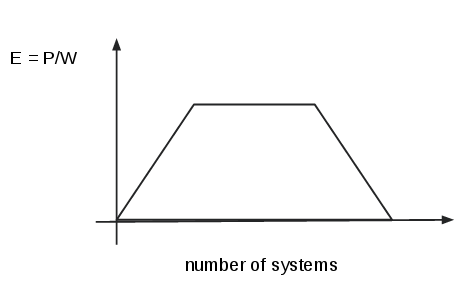
\includegraphics[width=0.75\textwidth]{images/graph_1.png}
\caption{Hypothesis of energy efficiency behaivor in embedded cluster}
\label{fig:1.2}
\end{figure}

The way we are going to test this hypotesis requires the following parts:


\begin{itemize}
\item Chose the rigth embedded platform 
\item Chose the right Distributed System comunication and compute protocol
\item Chose the right Operating System for the system (HW and comunication protocol) 
\item Crate embedded clusters to measure energy efficiency
\item Improve comunication protocol for embedded and IoT systems
\item Implement solution on real application ( greenhouse )
\end{itemize}

\section{Methodology}
\noindent

As described on the previus section the way we are trying to achive this
research is as follows: 


\begin{itemize}
\item Chose the rigth embedded platform: There are dozens of embedded and IoT
    platforms, this is why is necesary to make a deep analisys and choose the
    best platform that feed our needs. Is important to mention that in a real
    application like a greenhose the systems have an heterogenus architecture.
\item Chose the right Distributed System comunication and compute protocol.
    There are diferent kinds of distributed compute protocols. Part of this
    investigation is to detect the most reliable and suitable for our needs.
\item Chose the right Operating System for the system (HW and comunication
    protocol). Once we have selected the apropiate embedded platforms, another 
    varible in this investigation is the number of Operating
    Systems. Either if is a microkernel or a monolotic kernel architecture
    there are more than a dozen of choises for the current embedded platforms
    exist on the market (the only requirement is that they have a microprocesor
    instead of a microcontroller)
\item Crate embedded clusters to measure energy efficiency. Once we have find
    the best configuration ( HW + OS + Conumication Protocol ) and test thi set
    up has the higher energy efficiency, we can start to create a cluster of
    embedded systems. THe growth of th cluster will be by 2 ( 2,4,6,8,10..) ;
    measuring at the same time the energy efficency of the system.
\item Improve distributed technology for embedded and IoT systems. We will be
    focus on find improvements on the distributed technology (compute
    protocol, Operating System, Power and Performance) in order to make it part
    of world wide standards.
\item Implement solution on real application ( greenhouse ). In order to test
    or hypotesis in a real application we will implent it on a real
    greenhouse. Proving that the solution give an embedded system the power of
    reliability and availability without the need of external and expensive servers 
\end{itemize}


\clearpage
